\section{ニコ書を支えるイカ}

ニコ書チームでは過去にイカが大流行したことがありました。
きっかけは、ある日誰かがコンビニで買ってきた裂きイカを、みんなでつまんだことに始まります。
1袋はあっという間になくなり、その日だけで3袋追加で買った記憶があります。
ブームが決定的になったのは、味が濃くて歯ごたえも強い「函館こがね」を投入した瞬間でした。

\subsection{イカ基金}

初日のイカの消費量を考慮した結果、コンビニの裂きイカではコストが高すぎると分かりました。
そこでイカ基金を設立し、裂きイカ業者から直接大量購入する方法を取りました。
給料日に一口1000円で資金を徴収し、イカの共同購入と在庫管理をする担当者を置きました。

一度の注文で、裂きイカを中心に、イカフライやスルメなども混ぜ、約5キロほど購入します。
大きな段ボール箱が会社に届きチームに運ばれてきます。
届いたイカはとりあえず開封され、食い荒らされます。
スルメを噛みながら仕事をし、休憩がてら裂きイカを食い、イカフライをつまみながら朝会をし、
この量をだいたい半月で消費します。

\begin{figure}[H]
\centering
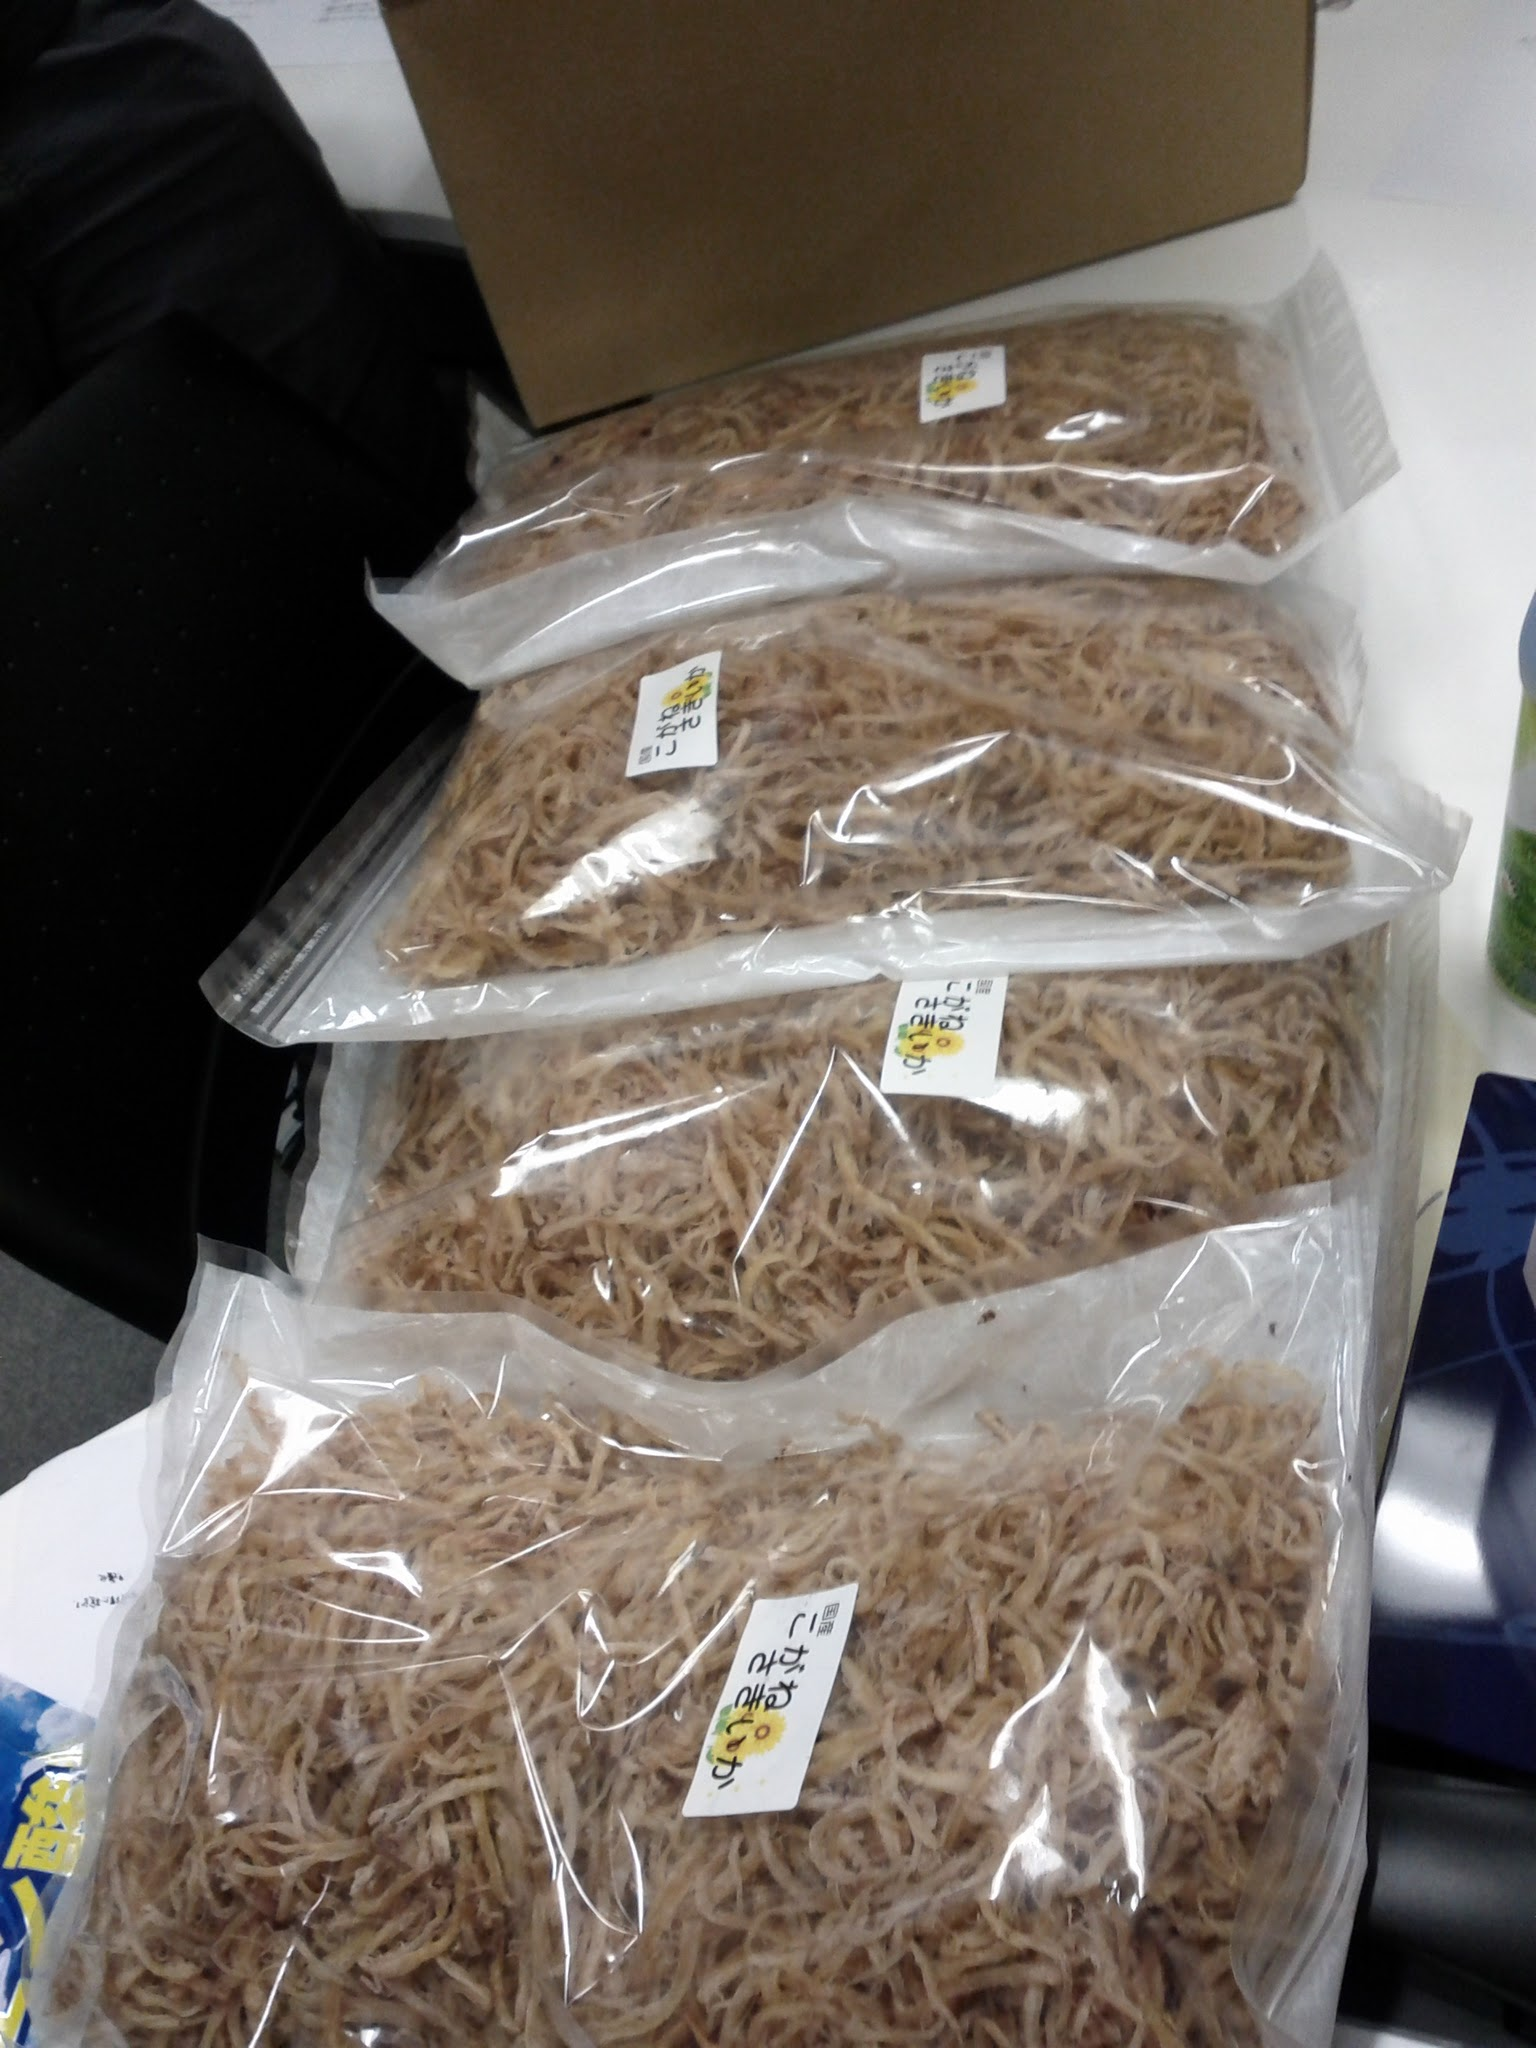
\includegraphics[width=0.7\textwidth]{../images/ika.jpg}
\caption{届いたばかりのイカ}
\end{figure}

\subsection{イカの効果}

イカそのものは、低カロリー・低脂肪・高タンパクと太りにくく、
不足しがちな亜鉛やビタミンを多く含んだ理想的な食材です。
ただし、料理法によって高カロリーか高塩分のどちらかになるので食べ過ぎに注意しましょう。
だいぶ太りました。

イカと言ったらやっぱりあの硬さです。
硬いものを噛み続けることは、脳の満腹中枢を刺激し、少量でも満腹を感じるようになります。
噛むことはストレス解消にもなるので、ストレスの多いこの仕事では、
イカを噛みながら仕事をすることでストレスの上昇を抑え、集中力を長く保つことに繋がります。
ただ顎関節症には気をつけましょう。柔らかいイカから慣らしましょう。

イカの最大の効果はその臭いです。
我々はイカの臭いとある種の記憶が密接に結びついており、
パブロフの犬の実験と同様に、イカの臭いにより身体的/精神的な条件反射が起こります。

すなわち、擬似的に賢者モードを発動することができるのです。
賢者モード中は思考がクリアになり、ストレスから開放され、
集中力が増し、仕事には最適な精神状態になります。
イカによる擬似賢者モードの時に、今まで全く気づかなかったバグやテストの漏れに気づくことが多々ありました。

\subsection{イカブームの終焉}

イカ基金の最大の敵は周囲の反発でした。
利点であるイカ臭さを理解できない無粋な大人たちが、イカ臭いからやめろと言ってくるのです。
この時は「我々のチームは イカがあろうがなかろうが
最初からイカ臭い」という主張により事なきを得ました。

しかし、こうまでして保護したイカブームもある日突然終了してしまいました。
それは、韓国土産でもらった韓国のさきイカを開封した瞬間でした。
あたりに漂う強烈なイカ臭さとは別種の腐ったような臭い、
ゴムのような気味の悪い歯ごたえ、妙に酸っぱくてイカの存在感を感じない味。
一言で言うと強烈に不味くて、誰もが「しばらくイカは見たくない・・・」という状況になりました。
結局誰も手を付けないまま、大量のカビが生えるまで放置され、カビだらけの袋を捨てると共にイカブームは終焉しました。

とは言うものの、今でもたまにコンビニのイカを買ってきて、みんなでつまんだりしています。
